\documentclass[prl,twocolumn,english,superscriptaddress,floatfix]{revtex4}
\usepackage[utf8]{inputenc}
\usepackage{graphicx}
\usepackage{float}
\usepackage{amsmath,amssymb,amstext}

\begin{document}

\title{How to write a PRL style paper in Latex}
\author{Kater Murch}
\affiliation{Department of Physics, Washington University, St.\ Louis, Missouri 63130}
%\author{Second Author}
%\affiliation{Department of Physics, Washington University, St.\ Louis, Missouri 63130}

\date{\today}

\begin{abstract}
The purpose of this paper is to serve as the simplest possible template for writing lab reports in the form of an APS manuscript. Special attention is paid to inserting figures, managing references, and inserting equations.
\end{abstract}
\maketitle

Start your paper with an introduction. You might find it necessary to type in an equation. This is done using the \$ sign.  
%note that if you want to print a $, you need to put a slash in front of it.
An example of an in-line equation is $f(\theta) = e^{i\theta}$.  You can also make equations that stand alone as their own line of text:
\begin{equation}
f(x) = \frac{3 x^2 + \sqrt{2}}{2 \pi}.  \label{firstequation}
\end{equation}
Equation (\ref{firstequation}) is a an example of a numbered equation that I can reference later in the text.  The numbering is taken care of automatically.

The second thing you will need to do is insert a figure.  First upload the file into the overleaf files location. I prefer to use .pdf figures, but other formats will work too. Figure \ref{figboxcircle} is an example of inserting a figure into a latex document. The location of the figure will float around the paper, usually taking the best possible location, but sometimes ending in a frustrating part of the document. It won't show up before where you place it in the text.

\begin{figure}
\begin{center}
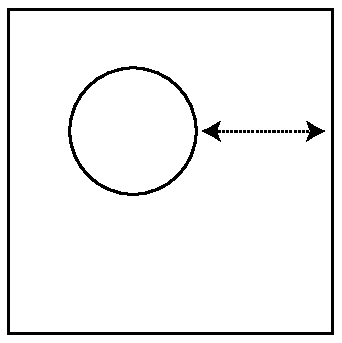
\includegraphics[width = 0.3\textwidth]{myfigure.pdf}
\end{center}
\caption{ This is the caption for the figure.}
\label{figboxcircle}
\end{figure}

The last thing you'll want to do is include references. Latex makes this really easy (well sorta easy).  First you need to create a .bib file with the reference information.  This way you can cite the latest research \cite{seig17,bert17}.

\bibliography{myrefs}

\end{document}
